\section{Результаты}

\subsection{Результаты для исходных данных}

Каждому датчику в чипе были присвоены координаты в зависимости от канала и номера ячейки. Датчик получивший данные из канала $j(1 \leq j \leq 8)$ и находящийся в ячейке $i(1 \leq j \leq 1024)$ будет иметь координаты $i, j$. Рассматриваются данные датчиков

\begin{enumerate}
    \item С координатами (0, 631)
    \item С координатами (3, 646)
    \item С координатами (6, 657)
\end{enumerate}

\begin{figure}[H]
    \centering
    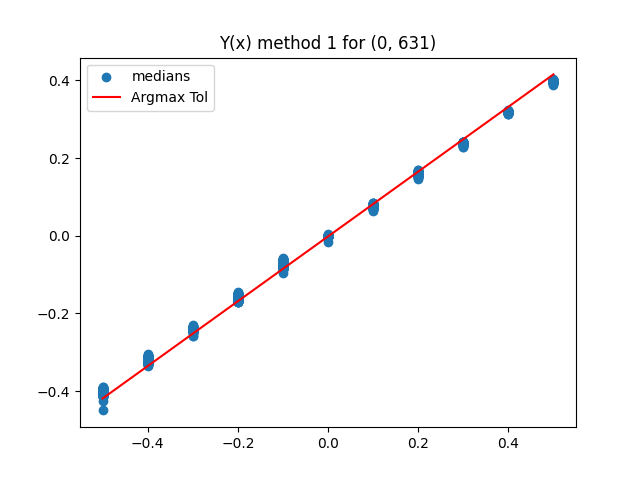
\includegraphics[width=0.7\linewidth]{image/0_631_method_1.png}
    \caption{Калибровочная прямая полученная первым методом для датчика (0, 631)}
    \label{fig:0_631_method_1}
\end{figure}

\begin{figure}[H]
    \centering
    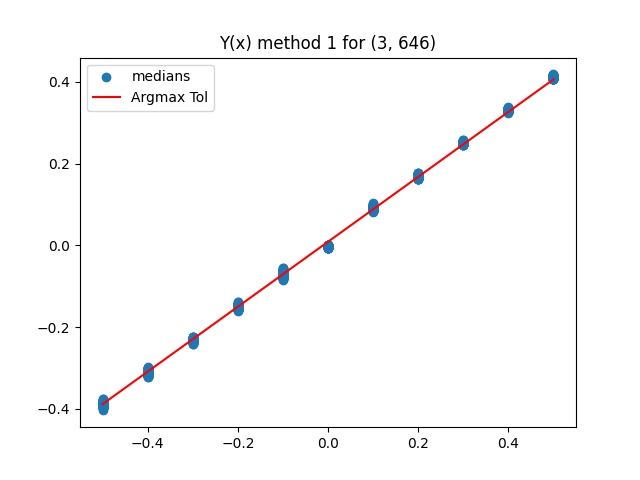
\includegraphics[width=0.7\linewidth]{image/3_646_method_1.png}
    \caption{Калибровочная прямая полученная первым методом для датчика (3, 646)}
    \label{fig:3_646_method_1}
\end{figure}

\begin{figure}[H]
    \centering
    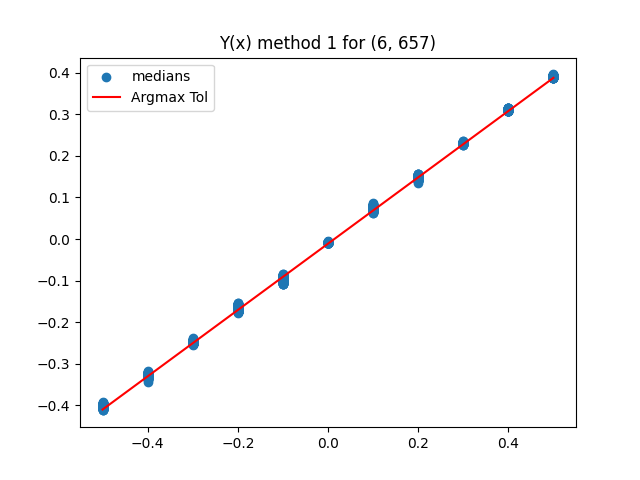
\includegraphics[width=0.7\linewidth]{image/6_657_method_1.png}
    \caption{Калибровочная прямая полученная первым методом для датчика (6, 657)}
    \label{fig:6_657_method_1}
\end{figure}

\begin{figure}[H]
    \centering
    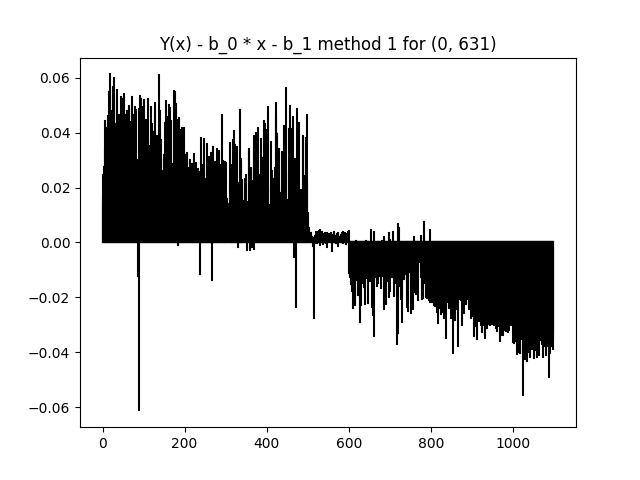
\includegraphics[width=0.7\linewidth]{image/0_631_method_1_difference.png}
    \caption{ Разность между данными и калибровочной прямой для первого метода и датчика (0, 631)}
    \label{fig:0_631_method_1_difference}
\end{figure}

\begin{figure}[H]
    \centering
    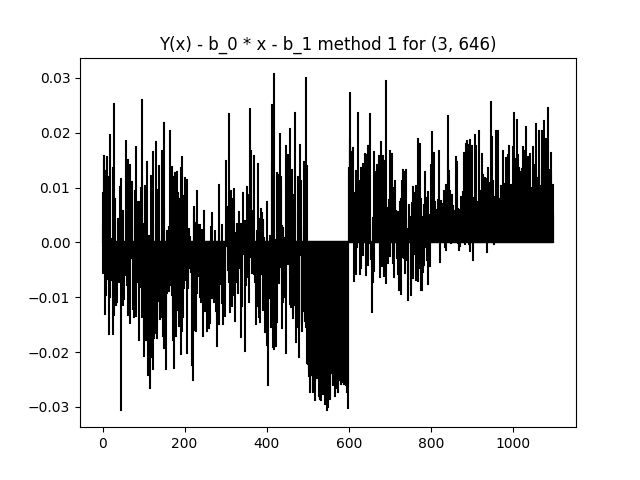
\includegraphics[width=0.7\linewidth]{image/3_646_method_1_difference.png}
    \caption{ Разность между данными и калибровочной прямой для первого метода и датчика (3, 646)}
    \label{fig:3_646_method_1_difference}
\end{figure}

\begin{figure}[H]
    \centering
    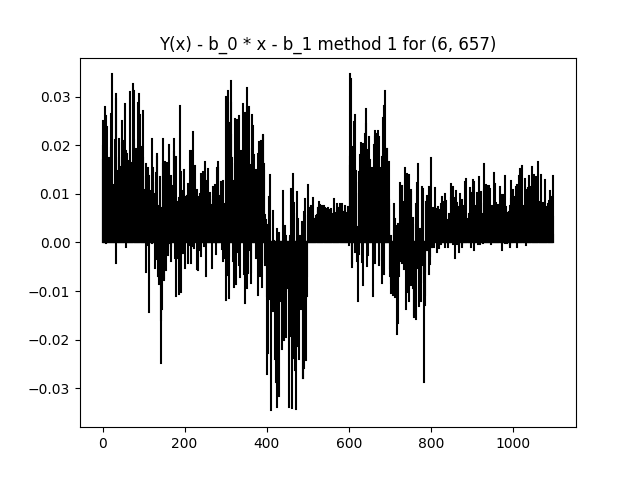
\includegraphics[width=0.7\linewidth]{image/6_657_method_1_difference.png}
    \caption{ Разность между данными и калибровочной прямой для первого метода и датчика (6, 657)}
    \label{fig:6_657_method_1_difference}
\end{figure}

\begin{figure}[H]
    \centering
    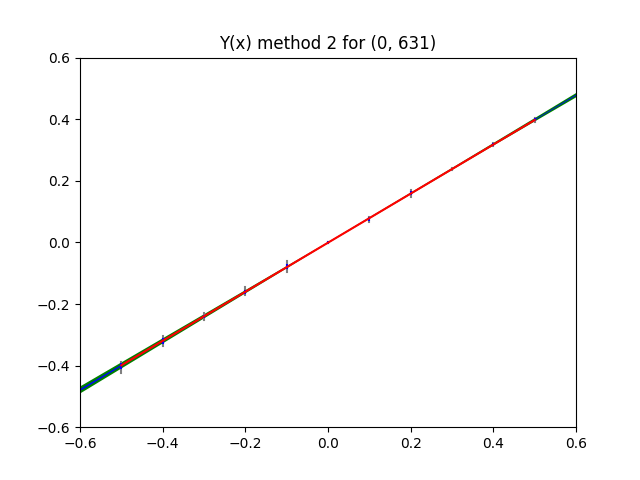
\includegraphics[width=0.7\linewidth]{image/0_631_method_2_corridor_joint_dependence.png}
    \caption{Калибровочная прямая полученная вторым методом для датчика (0, 631), обозначена красным цветом. Твины обозначены серым и черным цветом. Корридоры совместности Tol и $Tol_{ex}$ обозначены синим и зеленым цветом}
    \label{fig:0_631_method_2}
\end{figure}

\begin{figure}[H]
    \centering
    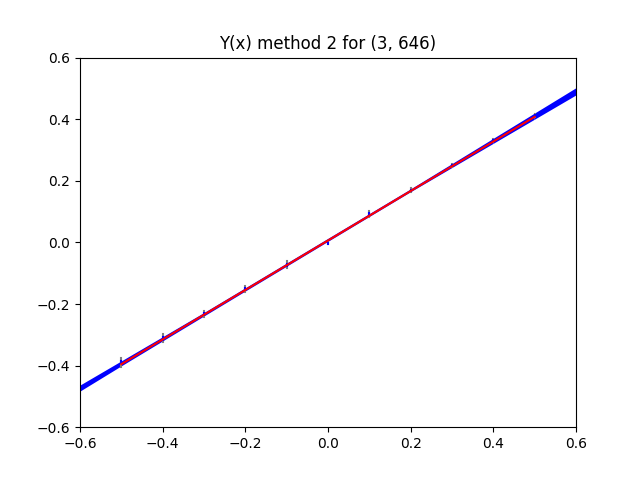
\includegraphics[width=0.7\linewidth]{image/3_646_method_2_corridor_joint_dependence.png}
    \caption{Калибровочная прямая полученная вторым методом для датчика (3, 646), обозначена красным цветом. Твины обозначены серым и черным цветом. Корридоры совместности Tol и $Tol_{ex}$ обозначены синим и зеленым цветом}
    \label{fig:3_646_method_2}
\end{figure}

\begin{figure}[H]
    \centering
    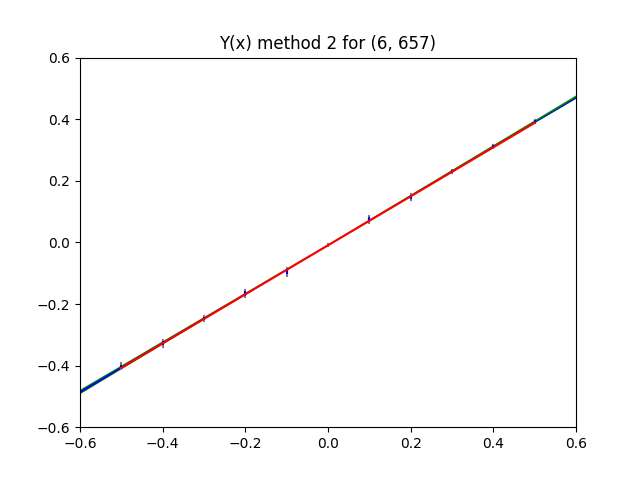
\includegraphics[width=0.7\linewidth]{image/6_657_method_2_corridor_joint_dependence.png}
    \caption{Калибровочная прямая полученная вторым методом для датчика (6, 657), обозначена красным цветом. Твины обозначены серым и черным цветом. Корридор совместности Tol обозначен синим цветом}
    \label{fig:6_657_method_2}
\end{figure}

\begin{figure}[H]
    \centering
    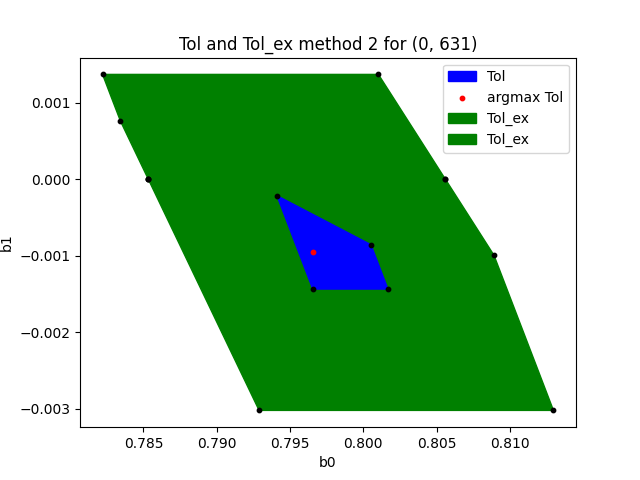
\includegraphics[width=0.7\linewidth]{image/0_631_method_2.png}
    \caption{Tol и $Tol_{ex}$ для датчика (0, 631)}
    \label{fig:0_631_tol}
\end{figure}

\begin{figure}[H]
    \centering
    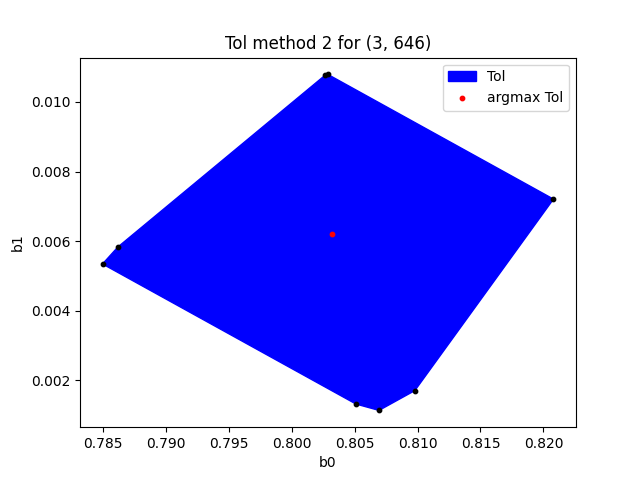
\includegraphics[width=0.7\linewidth]{image/3_646_method_2.png}
    \caption{Tol и $Tol_{ex}$ для датчика (3, 646)}
    \label{fig:3_646_tol}
\end{figure}

\begin{figure}[H]
    \centering
    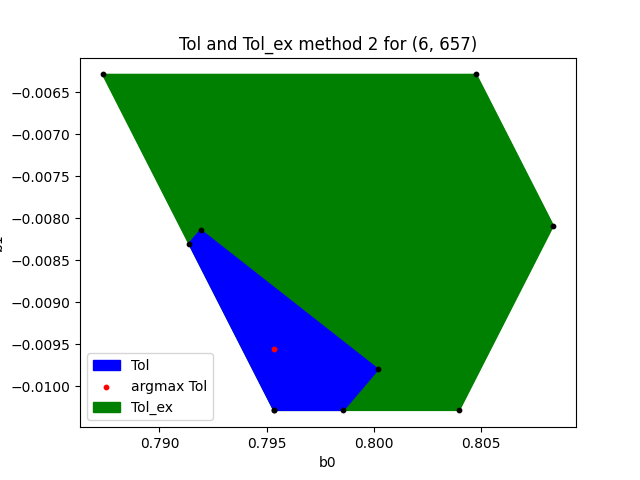
\includegraphics[width=0.7\linewidth]{image/6_657_method_2.png}
    \caption{Tol для датчика (6, 657)}
    \label{fig:6_657_tol}
\end{figure}

\begin{table}[H]
    \centering
    \begin{tabular}{|c|c|c|c|c|}
        \hline
         Координаты датчика &  Метод &  $\beta_0$ & $\beta_1$ & Количество модификаций\\ \hline
         (0, 631) & 1 & 0.8346 & -0.0018 & 1097 \\ \hline
         (0, 631) & 2 & 0.7966 & -0.0009 & 0 \\ \hline
         (3, 646) & 1 & 0.7948 & 0.0086 & 1092 \\ \hline
         (3, 646) & 2 & 0.8032 & 0.0062 & 30 \\ \hline
         (6, 657) & 1 & 0.7980 & -0.0112 & 1094 \\ \hline
         (6, 657) & 2 & 0.7953 & -0.0096 & 14 \\ \hline
    \end{tabular}
    \caption{Численные результаты}
    \label{tab:results}
\end{table}

\subsection{Результаты для упрощенных синтетических данных}

\begin{figure}[H]
    \centering
    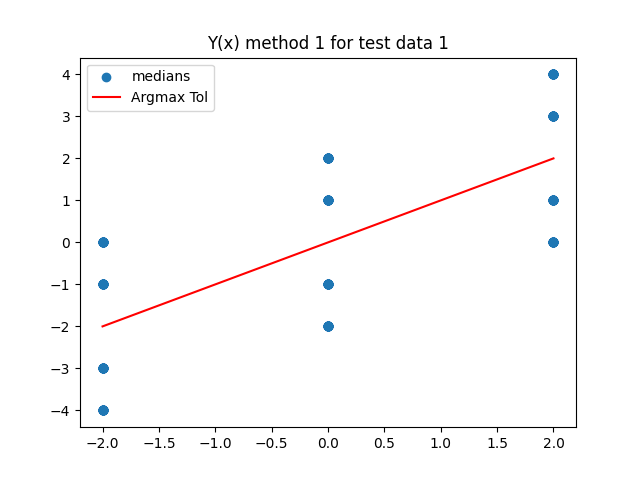
\includegraphics[width=0.7\linewidth]{image/test_1_method_1.png}
    \caption{Калибровочная прямая полученная первым методом для синтетических данных 1}
    \label{fig:test_1_method_1}
\end{figure}

\begin{figure}[H]
    \centering
    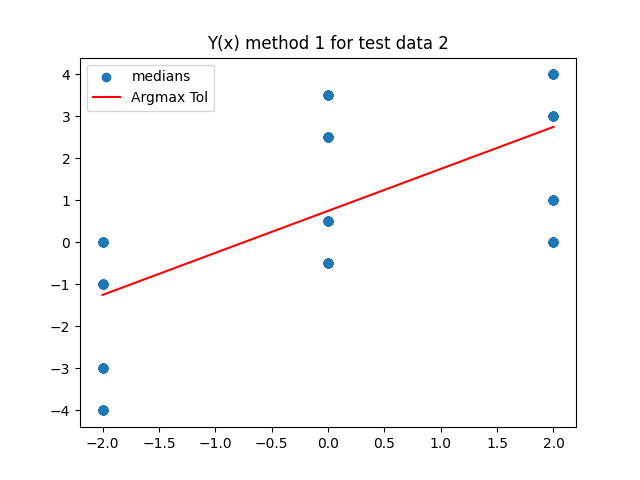
\includegraphics[width=0.7\linewidth]{image/test_2_method_1.png}
    \caption{Калибровочная прямая полученная первым методом для синтетических данных 2}
    \label{fig:test_2_method_1}
\end{figure}

\begin{figure}[H]
    \centering
    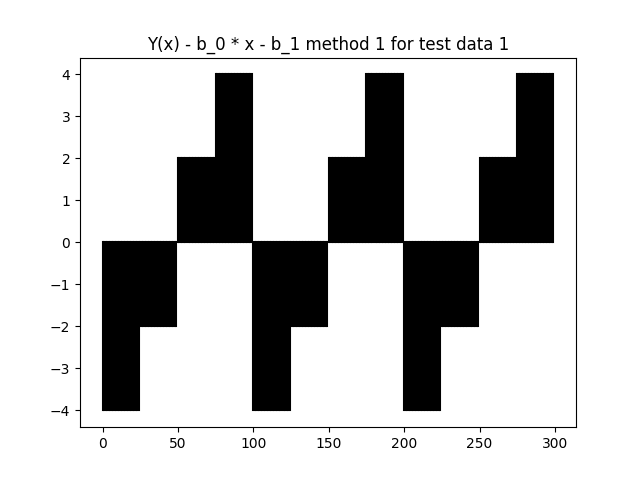
\includegraphics[width=0.7\linewidth]{image/test_1_method_1_difference.png}
    \caption{Разность между данными и калибровочной прямой для первого метода и синтетических данных 1}
    \label{fig:test_1_method_1_difference}
\end{figure}

\begin{figure}[H]
    \centering
    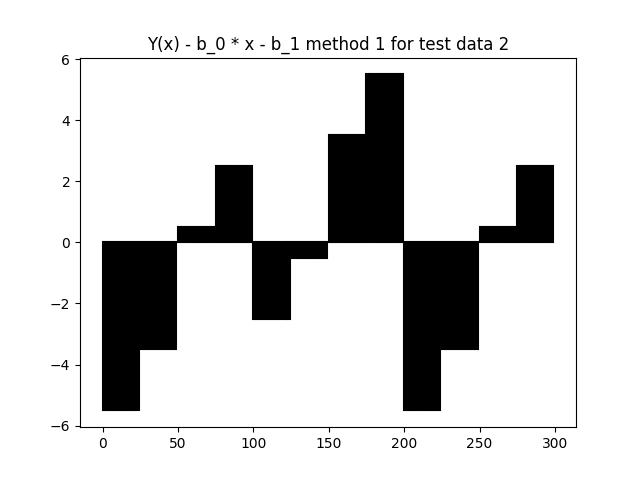
\includegraphics[width=0.7\linewidth]{image/test_2_method_1_difference.png}
    \caption{Разность между данными и калибровочной прямой для первого метода и синтетических данных 2}
    \label{fig:test_2_method_1_difference}
\end{figure}

\begin{figure}[H]
    \centering
    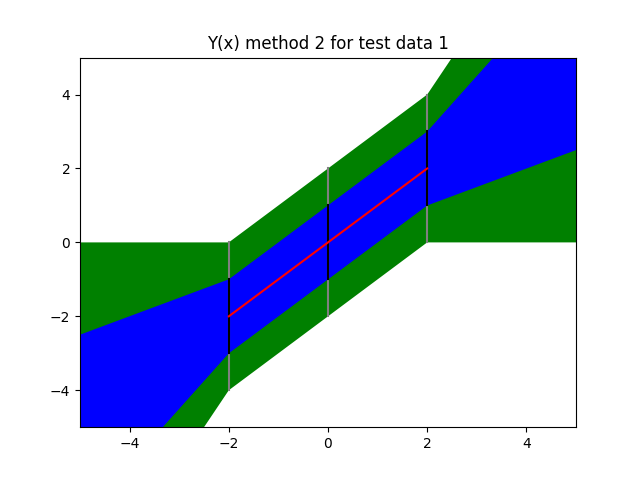
\includegraphics[width=0.7\linewidth]{image/test_1_method_2_corridor_joint_dependence.png}
    \caption{Калибровочная прямая полученная вторым методом для синтетических данных 1, обозначена красным цветом. Твины обозначены серым и черным цветом. Корридоры совместности Tol и $Tol_{ex}$ обозначены синим и зеленым цветом}
    \label{fig:test_1_method_2_corridor_joint_dependence}
\end{figure}

\begin{figure}[H]
    \centering
    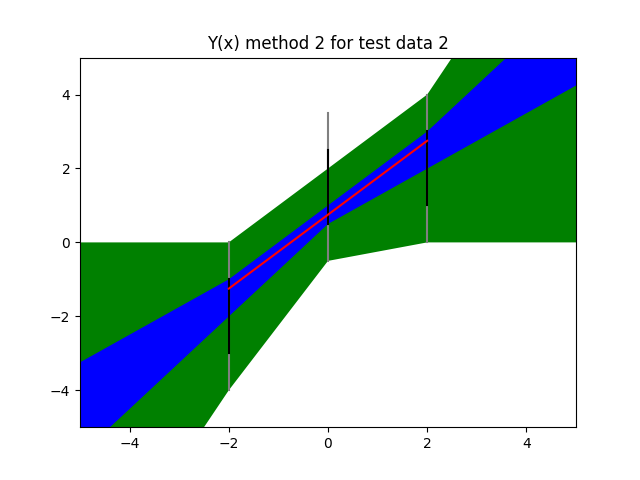
\includegraphics[width=0.7\linewidth]{image/test_2_method_2_corridor_joint_dependence.png}
    \caption{Калибровочная прямая полученная вторым методом для синтетических данных 2, обозначена красным цветом. Твины обозначены серым и черным цветом. Корридоры совместности Tol и $Tol_{ex}$ обозначены синим и зеленым цветом}
    \label{fig:test_2_method_2_corridor_joint_dependence}
\end{figure}

\begin{figure}[H]
    \centering
    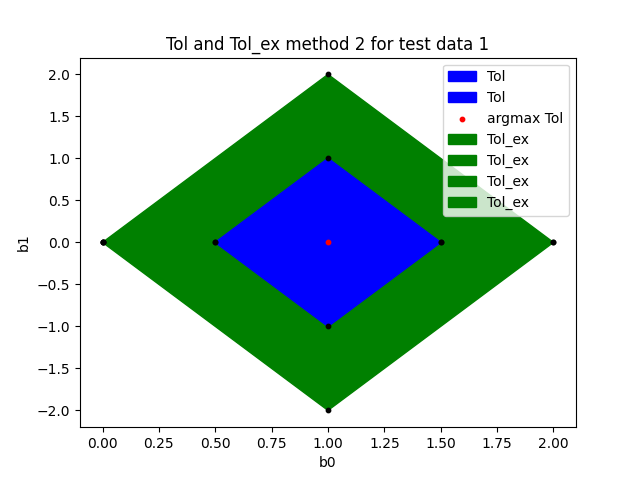
\includegraphics[width=0.7\linewidth]{image/test_1_method_2.png}
    \caption{Tol и $Tol_{ex}$ для синтетических данных 1}
    \label{fig:test_1_method_2}
\end{figure}

\begin{figure}[H]
    \centering
    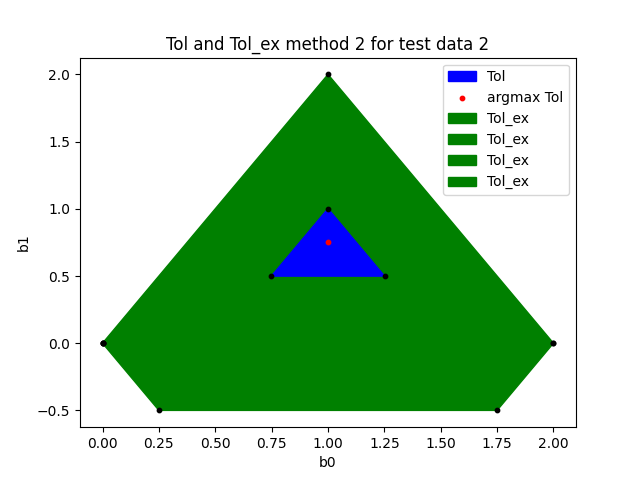
\includegraphics[width=0.7\linewidth]{image/test_2_method_2.png}
    \caption{Tol и $Tol_{ex}$ для синтетических данных 2}
    \label{fig:test_2_method_2}
\end{figure}